\section{Các chức năng chính}
Dưới đây là danh sách các yêu cầu chức năng của hệ thống, được phân loại theo từng module chức năng. Mỗi module đại diện cho một nhóm chức năng liên quan, hỗ trợ các hoạt động học tập, giảng dạy và quản lý hệ thống.

\subsection{Quản lý tài khoản (Thành viên đảm nhiệm: Phạm Thi)}
Module này cung cấp các chức năng liên quan đến đăng nhập, xác thực và quản lý thông tin cá nhân của người dùng.
\begin{itemize}[label=--]
    \item Đăng nhập vào hệ thống bằng email/mật khẩu hoặc tài khoản Google (Role: Sinh viên, Giảng viên, Quản trị viên).
    \item Làm mới token xác thực khi phiên đăng nhập hết hạn (Role: Sinh viên, Giảng viên, Quản trị viên).
    \item Xác minh email và gửi lại mã xác minh nếu cần (Role: Sinh viên, Giảng viên, Quản trị viên).
    \item Đặt lại mật khẩu khi quên mật khẩu (Role: Sinh viên, Giảng viên, Quản trị viên).
    \item Cập nhật thông tin cá nhân (tên, ngày sinh, ảnh đại diện) (Role: Sinh viên, Giảng viên, Quản trị viên).
    \item Xem thông tin hồ sơ cá nhân (ID, tên, email, MSSV/MSCB, ngày sinh, vai trò) (Role: Sinh viên, Giảng viên, Quản trị viên).
\end{itemize}

\begin{figure}[H]
    \centering
    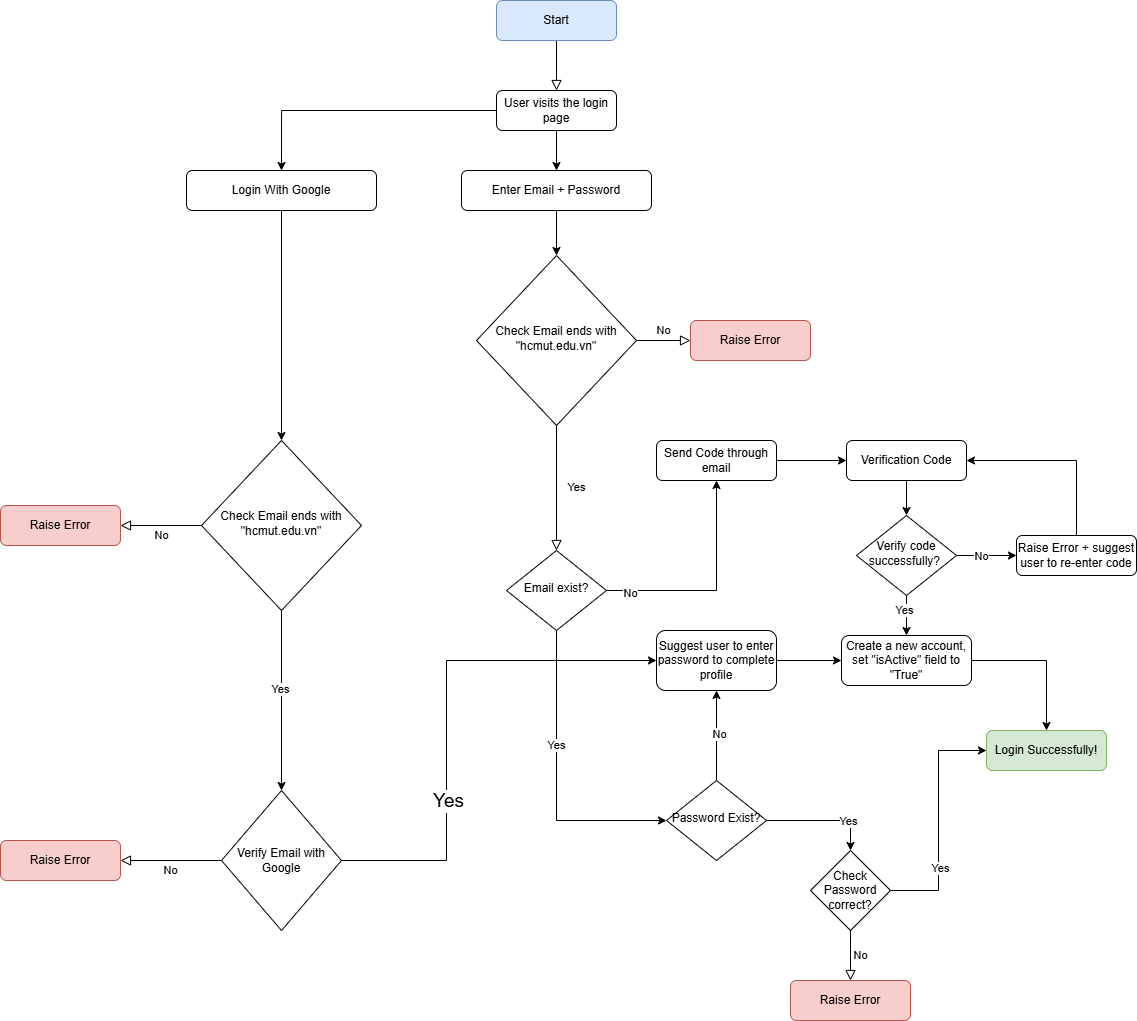
\includegraphics[width=0.9\linewidth]{images/Quan_ly_tai_khoan/authenFlow.drawio.png}
    \caption{Flow Định danh tài khoản}
    \label{fig:enter-label}
\end{figure}

\subsection{Quản lý khóa học (Thành viên đảm nhiệm: Phạm Thi/Tuấn Anh)}
Module này hỗ trợ quản lý thông tin khóa học, bao gồm tạo, xem, cập nhật và xóa dữ liệu liên quan.
\begin{itemize}[label=--]
    \item Xem danh sách khóa học (đã đăng ký hoặc đang phụ trách, hỗ trợ phân trang và tìm kiếm) (Role: Sinh viên, Giảng viên).
    \item Xem chi tiết khóa học (số lượng sinh viên, bài học, bài tập, tài liệu, tiến độ học tập) (Role: Sinh viên, Giảng viên).
    \item Xem thông tin Giảng viên của khóa học (Role: Sinh viên).
    \item Cập nhật mục tiêu học tập và ảnh khóa học (Role: Giảng viên).
    \item Tạo khóa học mới (đơn lẻ hoặc nhiều khóa) (Role: Quản trị viên).
    \item Cập nhật thông tin khóa học (tên, tín chỉ, học kỳ) (Role: Quản trị viên).
    \item Xóa khóa học cùng dữ liệu liên quan (Role: Quản trị viên).
    \item Xem danh sách khóa học có sẵn của HCMUT (Role: Quản trị viên).
    \item Xem khóa học truy cập gần đây nhất qua dashboard (Role: Sinh viên).
\end{itemize}

\subsection{Quản lý bài học (Thành viên đảm nhiệm: Phạm Thi/Tuấn Anh)}
Module này cho phép tạo, chỉnh sửa và quản lý bài học trong khóa học.
\begin{itemize}[label=--]
    \item Xem danh sách bài học trong khóa học (Role: Sinh viên).
    \item Tạo bài học mới (Role: Giảng viên).
    \item Cập nhật bài học (tiêu đề, mô tả, mục tiêu học tập) (Role: Giảng viên).
    \item Xóa bài học cùng tài liệu liên quan (Role: Giảng viên).
    \item Thêm tài liệu vào bài học (Role: Giảng viên).
    \item Xem chi tiết bài học và danh sách tài liệu liên quan (Role: Giảng viên).
\end{itemize}

\subsection{Quản lý bài tập (Thành viên đảm nhiệm: Tuấn Anh)}
Module này hỗ trợ quản lý bài tập dạng quiz và lập trình, bao gồm tạo, xem và nộp bài.
\begin{itemize}[label=--]
    \item Xem danh sách bài tập trong khóa học (chỉ bài tập đã mở) (Role: Sinh viên).
    \item Xem chi tiết bài tập dạng quiz hoặc lập trình (câu hỏi, yêu cầu, test cases) (Role: Sinh viên, Giảng viên).
    \item Tạo bài tập dạng quiz hoặc lập trình (Role: Giảng viên).
    \item Cập nhật thông tin bài tập dạng quiz hoặc lập trình (Role: Giảng viên).
    \item Xóa bài tập dạng quiz hoặc lập trình (Role: Giảng viên).
    \item Gửi câu hỏi tới trợ lý lập trình và xem lịch sử hội thoại (Role: Sinh viên).
    \item Nộp bài quiz và xóa câu trả lời để làm lại (Role: Sinh viên).
    \item Xem danh sách sự kiện bài tập sắp tới qua lịch học (Role: Sinh viên, Giảng viên).
\end{itemize}

\subsection{Quản lý lộ trình học tập (Thành viên đảm nhiệm: Phạm Thi)}
Module này cung cấp các chức năng liên quan đến lộ trình học tập cá nhân hóa và bài học đề xuất.
\begin{itemize}[label=--]
    \item Xem lộ trình học tập cá nhân hóa và danh sách bài học đề xuất (Role: Sinh viên).
    \item Xóa lộ trình học tập cá nhân (Role: Sinh viên).
    \item Xem chi tiết bài học đề xuất (tiêu đề, mục tiêu, nội dung, tiến độ) (Role: Sinh viên).
    \item Đánh dấu hoặc bỏ đánh dấu bài học đề xuất (Role: Sinh viên).
    \item Yêu cầu tạo lộ trình học tập dựa trên mục tiêu và khóa học (Role: Sinh viên).
    \item Tái tạo nội dung bài học dựa trên vấn đề đã xác định (Role: Sinh viên).
    \item Nhận gợi ý mục tiêu học tập từ hệ thống (Role: Sinh viên).
    \item Xem tài liệu của module trong lộ trình học tập (Role: Sinh viên).
    \item Tạo bài quiz dựa trên nội dung module (Role: Sinh viên).
\end{itemize}

\subsection{Theo dõi tiến độ học tập (Thành viên đảm nhiệm: Phạm Thi)}
Module này hỗ trợ theo dõi và đánh giá tiến độ học tập của sinh viên.
\begin{itemize}[label=--]
    \item Nhận đánh giá tiến độ học tập theo chuẩn Rubric (Role: Sinh viên).
    \item Cập nhật thời gian học cho bài học đề xuất (Role: Sinh viên).
    \item Xem phân tích tiến độ học tập trong khóa học hoặc bài học cụ thể (Role: Sinh viên).
    \item Xem điểm số của sinh viên trong khóa học (tên, email, MSSV, điểm trung bình) (Role: Giảng viên).
    \item Xem điểm chi tiết của một bài tập cụ thể (Role: Giảng viên).
\end{itemize}

\subsection{Quản lý phản hồi (Thành viên đảm nhiệm: Phạm Thi)}
Module này cho phép gửi, xem và quản lý phản hồi trong hệ thống.
\begin{itemize}[label=--]
    \item Gửi phản hồi về hệ thống hoặc khóa học (tiêu đề, mô tả, đánh giá) (Role: Sinh viên, Giảng viên).
    \item Xem danh sách phản hồi (lọc theo tháng, năm, trạng thái, khóa học) (Role: Giảng viên, Quản trị viên).
    \item Cập nhật trạng thái phản hồi (pending, in\_progress, resolved) (Role: Quản trị viên).
    \item Xóa phản hồi khỏi hệ thống (Role: Quản trị viên).
\end{itemize}

\subsection{Quản lý người dùng (Thành viên đảm nhiệm: Phạm Thi)}
Module này cung cấp các chức năng quản lý thông tin và trạng thái người dùng trong hệ thống.
\begin{itemize}[label=--]
    \item Tạo người dùng mới (sinh viên, Giảng viên, quản trị viên) (Role: Quản trị viên).
    \item Đếm số lượng người dùng (tổng hoặc theo vai trò) (Role: Quản trị viên).
    \item Xem danh sách tất cả người dùng (lọc theo vai trò, trạng thái, tìm kiếm) (Role: Quản trị viên).
    \item Xem thông tin chi tiết của một người dùng cụ thể (Role: Quản trị viên).
    \item Cập nhật trạng thái người dùng (bật/tắt) (Role: Quản trị viên).
\end{itemize}

\subsection{Quản lý nhật ký đăng nhập (Thành viên đảm nhiệm: Phạm Thi)}
Module này hỗ trợ theo dõi và ghi nhận hoạt động đăng nhập của người dùng.
\begin{itemize}[label=--]
    \item Xem danh sách nhật ký đăng nhập (ID người dùng, vai trò, thời gian) (Role: Quản trị viên).
    \item Tạo bản ghi nhật ký đăng nhập mới (Role: Quản trị viên).
\end{itemize}

\subsection{Quản lý dashboard (Thành viên đảm nhiệm: Phạm Thi)}
Module này cung cấp tổng quan hoạt động cho người dùng qua giao diện dashboard.
\begin{itemize}[label=--]
    \item Xem tổng quan hoạt động giảng dạy (số lượng khóa học, bài học, sinh viên, bài tập) (Role: Giảng viên).
    \item Xem và thêm các hoạt động gần đây (tối đa 5 hoạt động) (Role: Sinh viên).
\end{itemize}